%slide di introduzione ai fondamenti di Document Type Definition
%frame 01
\begin{frame}
    \frametitle{Elementi per la definizione degli schemi xml}
    \framesubtitle{Principi Document Type Definition}
    \addtocounter{nframe}{1}

    \begin{block}{Esempio DTD}
        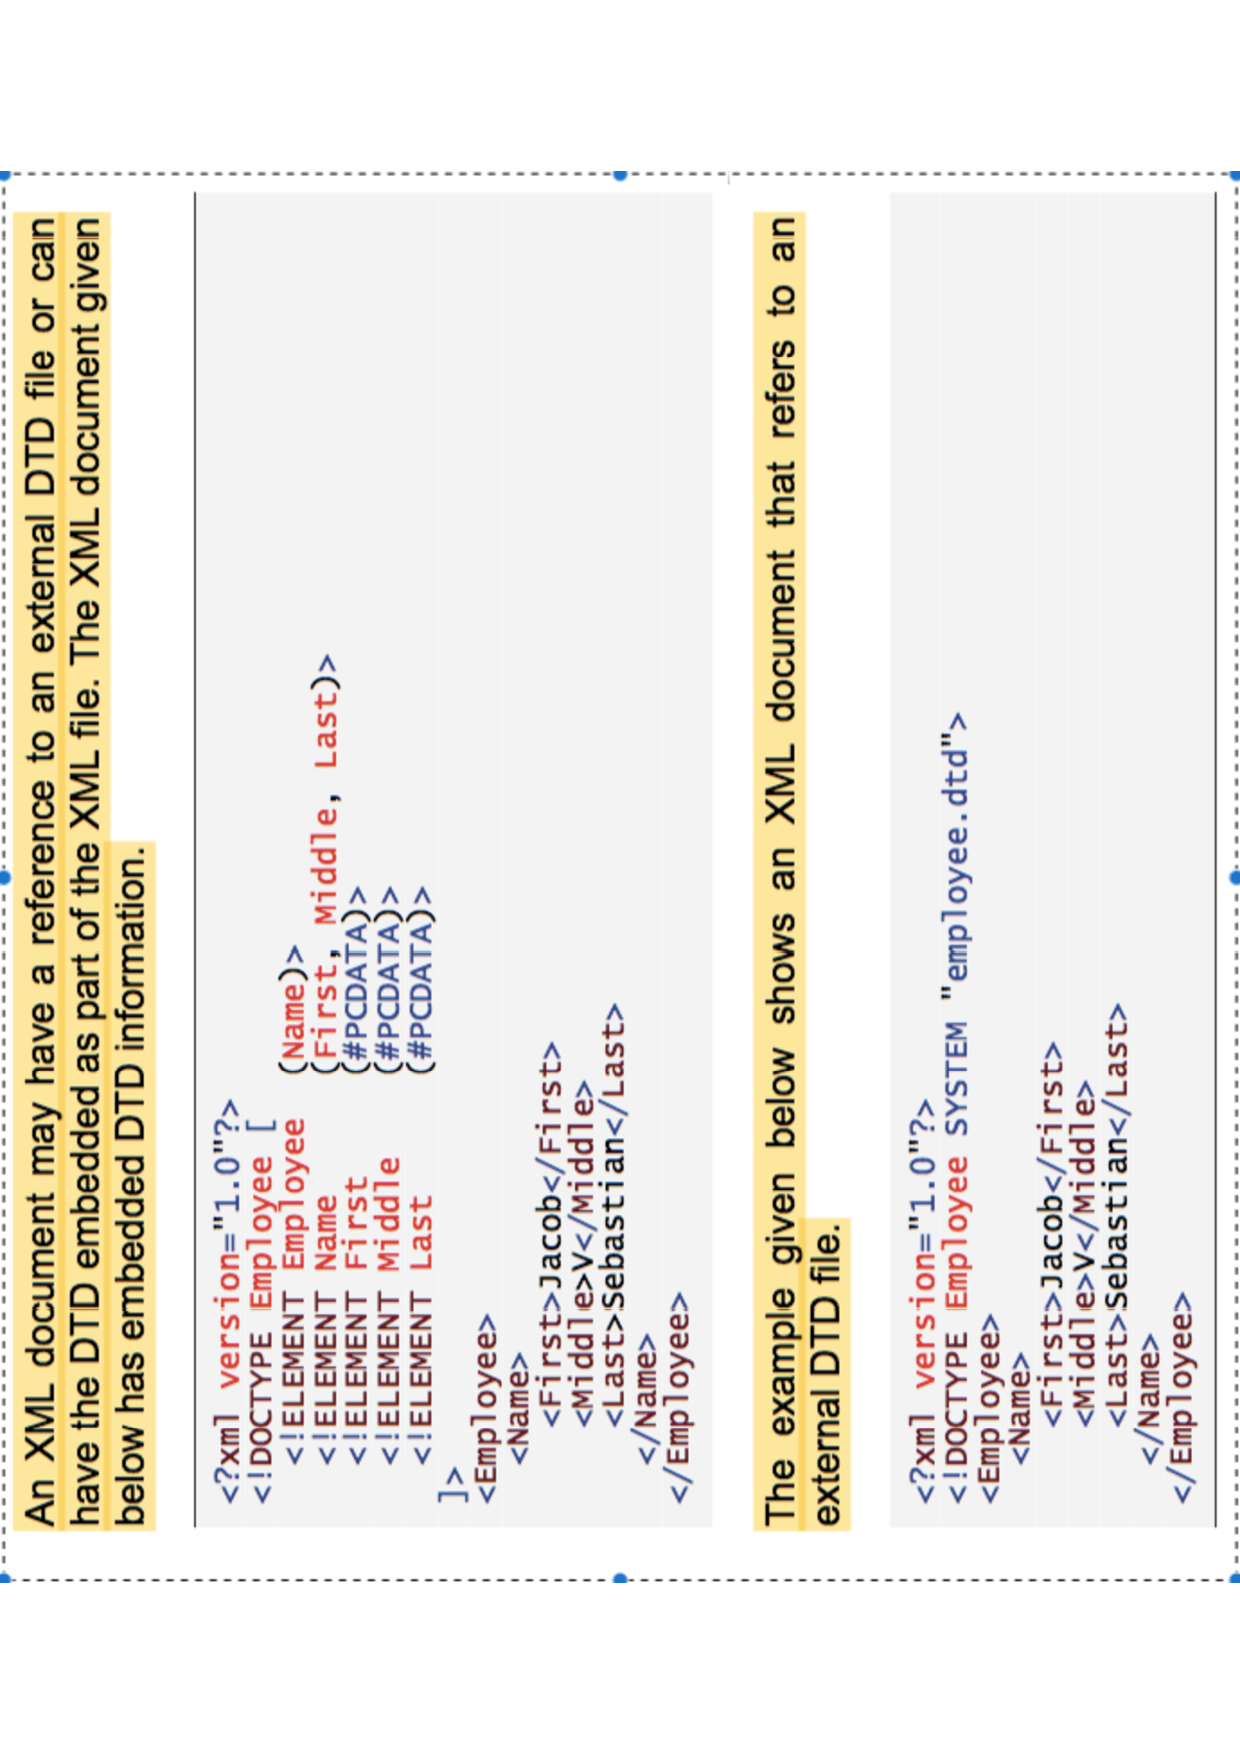
\includegraphics[width=.5\textwidth]{imgs/dtd_1.pdf}
    \end{block}
\end{frame}

\begin{frame}
    \frametitle{Elementi per la definizione degli schemi xml}
    \framesubtitle{Principi Document Type Definition}
    \addtocounter{nframe}{1}

    \begin{block}{Document Type Definition (DTD)}
        A document type definition describes the rule for an xml document structure, declaring the elements, attributes and entities that are part of the xml document
    \end{block}

\end{frame}

\begin{frame}
    \frametitle{Elementi per la definizione degli schemi xml}
    \framesubtitle{Principi Document Type Definition}
    \addtocounter{nframe}{1}

    \begin{block}{Document Type Definition (DTD)}
         For an xml document to be valid, it must be well formed and also satisfies the document type definitions specified by the document type declaration.
    \end{block}
\end{frame}

\begin{frame}
    \frametitle{Elementi per la definizione degli schemi xml}
    \framesubtitle{Principi Document Type Definition}
    \addtocounter{nframe}{1}

    \begin{block}{Document Type Definition (DTD)}
         For an xml document to be valid, it must be well formed and also satisfies the document type definitions specified by the document type declaration.
    \end{block}

    \begin{block}{well-formed document != valid document}
          any document that lacks a document type declaration may be well formed but cannot be valid.
    \end{block}
   
\end{frame}

\begin{frame}
    \frametitle{Elementi per la definizione degli schemi xml}
    \framesubtitle{Principi Document Type Definition}
    \addtocounter{nframe}{1}

    \begin{block}{Document Type Definition (DTD)}
          Document validation also aids file sharing since different applications that are
aware of the generally agreed upon document type definition can produce xml
document of similar structure and therefore easily communicate with each
other through data exchange.
    \end{block}
   
\end{frame}


\begin{frame}
    \frametitle{Elementi per la definizione degli schemi xml}
    \framesubtitle{Principi Document Type Definition}
    \addtocounter{nframe}{1}

    \begin{block}{Document Type Definition (DTD)}
         included in the document’ prolog
    \end{block}

    \begin{block}{Root element and content}
        declare the root element and its content model (children elements)
    \end{block}
   
\end{frame}

\begin{frame}
    \frametitle{Elementi per la definizione degli schemi xml}
    \framesubtitle{Principi Document Type Definition}
    \addtocounter{nframe}{1}

    \begin{block}{Element Declaration (con figli)}
        \begin{center}\texttt{<!ELEMENT element-name (child-element1, child-element-2 ...)>}\end{center}
    \end{block}

    \begin{block}{Element Declaration (solo testo)}
    \begin{center}\texttt{<!ELEMENT element-name (\#PCDATA)>}\end{center}
    \end{block}
    \textit{Parsed character contents are plain texts with no child elements}
\end{frame}

\begin{frame}
    \frametitle{Elementi per la definizione degli schemi xml}
    \framesubtitle{Principi Document Type Definition}
    \addtocounter{nframe}{1}

    \begin{block}{Child Element Declaration}
        A child element declaration is done in the same way as the root element declaration using the <!ELEMENT > tag
    \end{block}

    \begin{block}{Element Declaration (root)}
     root element declaration must always come first.
    \end{block}
\end{frame}


\begin{frame}
    \frametitle{Elementi per la definizione degli schemi xml}
    \framesubtitle{Principi Document Type Definition}
    \addtocounter{nframe}{1}

    \begin{block}{Modificatori}
        Optional modifiers can also be used in element declarations to specify the
        number of times a child element may appear.
    \end{block}

    \begin{block}{Modificatori}
     + One or more occurrences\\ 
     ? Zero or one occurrence\\
     * Zero or more occurrences\\
    \end{block}
\end{frame}

\begin{frame}
    \frametitle{Elementi per la definizione degli schemi xml}
    \framesubtitle{Principi Document Type Definition}
    \addtocounter{nframe}{1}

    \begin{block}{Modificatori}
        \begin{center} \texttt{<!ELEMENT element-name (B, C)+ >} \end{center}
        \begin{center} \texttt{<!ELEMENT element-name (B+, C) >} \end{center}
        \begin{center} \texttt{<!ELEMENT element-name (B, C+) >} \end{center}
        \begin{center} \texttt{<!ELEMENT element-name (B+, C+) >} \end{center}
    \end{block}

    \begin{block}{Modificatori}
     If a child element must appear once then leave out the modifier.
    \end{block}
\end{frame}

\begin{frame}
    \frametitle{Elementi per la definizione degli schemi xml}
    \framesubtitle{Principi Document Type Definition}
    \addtocounter{nframe}{1}

    \begin{block}{Esercizio}
        - root: TEI
        - figli: header (obbligatorio una occorrenza); facsimile (opzionale una occorrenza); text (obbligatorio almeno una occorrenza)
        - header, facsimile, text hanno un content model testuale
    \end{block}

\end{frame}


\begin{frame}
    \frametitle{Elementi per la definizione degli schemi xml}
    \framesubtitle{Principi Document Type Definition}
    \addtocounter{nframe}{1}

    \begin{block}{choice declaration}
    \begin{center} \texttt{<!ELEMENT element_name (child_a | child_b) >} \end{center}
    \end{block}

    \begin{block}{Dichiarazione di Choice}
        indicating a choice of just one, out of the list
    \end{block}

\end{frame}

\begin{frame}
    \frametitle{Elementi per la definizione degli schemi xml}
    \framesubtitle{Principi Document Type Definition}
    \addtocounter{nframe}{1}

    \begin{block}{Attributi}
    \begin{center} an attribute is declared with \texttt{<!ATTLIST >} element \end{center}
    \end{block}

    \begin{block}{Attributi}
        An attribute is the property of an element that describes the element’s content.
    \end{block}

\end{frame}

\begin{frame}
    \frametitle{Elementi per la definizione degli schemi xml}
    \framesubtitle{Principi Document Type Definition}
    \addtocounter{nframe}{1}

    \begin{block}{Attributi}
    \begin{center} \texttt{<!ATTLIST Element-name Attr-name Attr-type Attr-state? default-value?>} \end{center}
    \end{block}

    \begin{block}{Attributi}
        ``Element-name'' is the name of the element
        ``Attr-name'' is the attribute to be declared.
        ``Attr-type'' specifies the expected attribute’s data type
        The ``Attr-state'' denota una tra i tre stati possibili di un attributo 
        ``default-value'' if provided is the value to be used if the attribute is not supplied
    \end{block}

\end{frame}

\begin{frame}
    \frametitle{Elementi per la definizione degli schemi xml}
    \framesubtitle{TABELLA dei tipi}
    \addtocounter{nframe}{1}

    \begin{block}{Tipi di attributi}
    
    \end{block}
\end{frame}



\begin{frame}
    \frametitle{Elementi per la definizione degli schemi xml}
    \framesubtitle{}
    \addtocounter{nframe}{1}

    \begin{block}{Stato di attributi}
     The state can be any of #IMPLIED (an optional attribute), #REQUIRED (a compulsory attribute) or #FIXED (a fixed value attribute that may not be changed) the value is provided as the default value. You cannot use the default-value with the #REQUIRED state as you must supply a value for the attribute.
    \end{block}
\end{frame}

% slide con choice per gli attributi

\begin{frame}
    \frametitle{Elementi per la definizione degli schemi xml}
    \framesubtitle{}
    \addtocounter{nframe}{1}

    \begin{block}{Mixed content - DTD}
    \begin{center}\texttt{<!ELEMENT element_name (#PCDATA|child_element)* >}\end{center}
    \end{block}

    \begin{block}{Mixed content XML}
    \begin{center}\texttt{<p>Ieri pomeriggio sono andato a <placeName>Pisa<placeName>, per un giro<p>}\end{center}
    \end{block}

\end{frame}


\begin{frame}
    \frametitle{Elementi per la definizione degli schemi xml}
    \framesubtitle{}
    \addtocounter{nframe}{1}

    \begin{block}{Esercizio}
        root: TEI
         figli: header(obbligatorio una volta sola) - facsimile(opzionale una volta sola) - testo(obbligatorio una o più volte)
         - testo è un mixed content con possibile elemento <seg>
         attributi: 
         - header: type:(fixed, CDATA ``intestazione''); lang(opzional, NMTOKEN)
         - facsimile: source:(obbligatorio)
         - testo: id(obbligatorio, contenuto id) type(opzionale contenuto testuale)
    \end{block}
\end{frame}



\begin{frame}
    \frametitle{Elementi per la definizione degli schemi xml}
    \framesubtitle{Principi Document Type Definition}
    \addtocounter{nframe}{1}

    \begin{block}{Empty elements}
    The only difference is that the child element name is substituted with the keyword “EMPTY”  
    \end{block}

    \begin{block}{Empy content}
    \begin{center}\texttt{<!ELEMENT element_name EMPTY>}\end{center}
    \end{block}


    \begin{block}{Empy content}
    \begin{center}\texttt{<lb />}\end{center}
    \end{block}
    
    

\end{frame}


\begin{frame}
    \frametitle{Elementi per la definizione degli schemi xml}
    \framesubtitle{Principi Document Type Definition}
    \addtocounter{nframe}{1}

    \begin{block}{Any elements}
 The content specification ``ANY'' when used in a declaration implies that any element as well as texts can be the child or content of the declared element.

    \end{block}

    \begin{block}{Any content}
    \begin{center}\texttt{<!ELEMENT element_name ANY >}\end{center}
    \end{block}
    
\end{frame}


\begin{frame}
    \frametitle{Elementi per la definizione degli schemi xml}
    \framesubtitle{Principi Document Type Definition}
    \addtocounter{nframe}{1}

    \begin{block}{Dichiarare il tipo del documento XML}
        The document type declaration is placed in the xml document prolog; between
         the xml declaration and the root element.

    \end{block}

    \begin{block}{Dichiarare il tipo del documento XML}
        re-usability reasons, and then link it to the xml document and any other xml document through its URL
    \end{block}

\end{frame}

\begin{frame}
    \frametitle{Elementi per la definizione degli schemi xml}
    \framesubtitle{Principi Document Type Definition}
    \addtocounter{nframe}{1}

    \begin{block}{DOCTYPE}
    \begin{center}\texttt{<!DOCTYPE root_element SYSTEM ``External DTD’s URL'' [Internal DTD ]>}\end{center}
    \begin{center}\texttt{<!DOCTYPE root_element [Internal DTD] >}\end{center}
    \begin{center}\texttt{<!DOCTYPE root_element SYSTEM “External_DTD’s URL” >}\end{center}
        
    \end{block}
    
\end{frame}

\begin{frame}
    \frametitle{Elementi per la definizione degli schemi xml}
    \framesubtitle{Principi Document Type Definition}
    \addtocounter{nframe}{1}

    \begin{block}{Esercizi}
    \begin{itemize}
        \item includere all'interno di un documento XML la dichiarazione del tipo e validare
        \item inserire nel prologo di un documento XML la dichiarazione del tipo di documento e validare.
    \end{itemize}
    \end{block}
    \textit{creare un file esterno con estensione .dtd e includerlo nel prologo XML.}
    
\end{frame}

\begin{frame}
    \frametitle{Elementi per la definizione degli schemi xml}
    \framesubtitle{Principi Document Type Definition}
    \addtocounter{nframe}{1}

    \begin{block}{Entity}
        per includere dati da diverse fonti DTD prevede l'uso di entità. Due tipologie di entità sono state definite: general entities e parameter entities.
    \end{block}

    \begin{block}{Entity: generiche e parametriche}
    \begin{itemize}
        \item le general entities vengono espanse nel documento XML
        \item parameter entities vengono espanse nel documento DTD
    \end{itemize}
    \end{block}
    \textit{creare un file esterno con estensione .dtd e includerlo nel prologo XML.}
    
\end{frame}

\begin{frame}
    \frametitle{Elementi per la definizione degli schemi xml}
    \framesubtitle{Principi Document Type Definition}
    \addtocounter{nframe}{1}

    \begin{block}{Entity}
    \begin{itemize}
        \item  Le general entities si possono classificare in interne ed esterne; che a loro volta possono essere parsed oppure unparsed.
        \item Le parameter entities si possono classificare in interne ed esterne; che  possono essere solo parsed.
    \end{itemize}
    \end{block}
    \textit{creare un file esterno con estensione .dtd e includerlo nel prologo XML.}
    
\end{frame}


% An xml document may include other xml documents and data from different
% sources, these sources are termed entities and an entity can be external or
% internal entity.

% Internal general entities help include special characters in an xml document,
% that would otherwise make an xml document become malformed if included
% literally.


% The syntax of usage is as described below:


% <!ENTITY entity_name “replacement_string” or “hexadecimal_code” >


% To use the entity name in the element content simply attach the ampersand to
% the beginning of the entity name and append the semi colon to the end like
% this; &entity_name;


% may include well formed xml elements.


% An xml document may be developed from other xml document located in
% different places and from different applications. This is made possible through
% the use of external general entities. Through which the external entities are
% inserted into the main xml document. The syntax for an external general entity
% is as described below: <!ENTITY entity_name SYSTEM “URL” > The URL
% points to the location of the external entity to be drawn into the main
% document.


% <!ENTITY External_fruits SYSTEM "fruits.xml" >


% Please note that an external entity cannot contain a document type declaration
% as it will conflict with the main xml document type declaration, but you may
% include a text declaration in an external parsed entity, if not the parser will
% naturally assume a “UTF-8” encoding for the external entity. General entities
% though declared in the DTD, must be used in the document and not in the
% DTD itself. Also for now, Mozilla, Netscape, Safari and Opera do not resolve
% entity references except the latest version of internet explorer.

% General entities defined in the document type definition must appear in the xml
% document content, becoming a part of the xml document. This is a limitation of
% general entities as they cannot be exclusively used as parameters in the
% document type definition.


% This is however addressed by parameter entities. Parameter entity usage
% syntax is as described below: <!ENTITY % entity_name “replacement_string”
% >


% In other words parameter entity references are part of the DTD but may not
% appear in the document content.


% More, a parameter entity reference is started with a percentage sign


% (%) and not with the ampersand, and terminated with a semi colon like shown
% below: %parameterEntityName;


% There are two types of parameter entity; the internal and the external
% parameter entities.


% Internal parameter entities are used much in the same way that the general
% entity references are used but they remain parts of the dtd and never appear
% in the document’s content. An internal parameter entity reference is
% represented as shown below: <!ENTITY % parameter_entity_name
% “replacement_content” >

% When a parameter entity is inserted in the dtd, the parameter entity is replaced
% with the replacement content at execution time.


% Internal parameter entities are declared in the dtd external subset


% This would make the dtd easier to develop and later maintained, if there are
% any changes to be made.


% A parameter entity that is only a part of a complete declaration like above
% cannot appear in the internal definition subset of a dtd and must be placed in
% the external definition subset and referred to.


% Note that the parameter entity reference ”%Event_info;” was declared before it
% was used, and that “sport_calendar.dtd” was referred to in the external dtd
% subset as described in document 5.3 below:


% External parameter entities enable the modularization and linking of document
% type definitions.


% with external parameter entities you can embed modularized document type
% definitions from different locations to form a single and more complete
% document type definition.

% The syntax for an external parameter entity is as described below:


% <!ENTITY % parameter_name SYSTEM “URL” > %parameter_name;


% using an external parameter entity reference as shown
